\section{Concept Identification Annotation Guidelines} \label{app:concept_guidelines}

In this section, we discuss the guidelines that we created for annotators to identify concepts critical to understanding a document.

\begin{itemize}
\setlength\itemsep{-1em}
\item \textbf{Label nouns and compound nouns that express a concept critical relevant for understanding.} In some cases, only the head of the noun phrase, i.e. the noun itself, is the concept, while in other cases, a larger part of the noun phrase should be labeled as a concept.
	\vspace{-3.5mm}
	\begin{itemize}
		\setlength\itemsep{-1em}
      		\item \textbf{Example}: Using the classic \underline{algorithms} of \underline{machine learning}, text is considered as a sequence of keywords.
     		 \item In this example, we label \textit{algorithms} as a concept, but not \textit{classic algorithms} or \textit{the classic algorithms}. On the other hand, the phrase \textit{machine learning} is a multi-word expression that represents a technical concept, so we must annotate the entire noun phrase in this case.
    	\end{itemize}
\item \textbf{Only label noun phrases as concepts.} For our annotations, please do not just annotate an adjective or adverb. Instead, you should include it as part of a noun phrase.
	\vspace{-3.5mm}
	\begin{itemize}
		\setlength\itemsep{-1em}
      		\item \textbf{Example}: A three-dimensional vortex presents identical \underline{perpendicular lines} at any given time.
    	\end{itemize}
\item \textbf{Label common nouns that are used in specific technical contexts.} In certain domains, normally common words acquire a technical meaning that warrant them being labeled as a concept.
	\vspace{-3.5mm}
	\begin{itemize}
		\setlength\itemsep{-1em}
      		\item \textbf{Example}: Machine learning is concerned with minimizing the \underline{loss} on unseen examples...a representative book was Nilsoon's \textit{Learning Machines}.
     		 \item In this example, \textit{loss} is a concept, as even though it is a common word, it is used in an uncommon, machine learning-specific context. On the other hand, \textit{book} is not a concept in this context.
    	\end{itemize}
\item \textbf{When a concept appears along with a prepositional phrase, label the full phrase.} Some nouns are followed by prepositional phrases describing the noun. For these, please label the entire phrase, including the preposition.
	\vspace{-3.5mm}
	\begin{itemize}
		\setlength\itemsep{-1em}
      		\item \textbf{Example}: Each section is perpendicular to its \underline{axis of rotation}...This area is usually called the \underline{core of the reverberator}.
    	\end{itemize}
\item \textbf{Annotate all distinct versions of concepts.} There are some expressions which, while they may overlap in word usage, represent different concepts. 
	\vspace{-3.5mm}
	\begin{itemize}
		\setlength\itemsep{-1em}
      		\item \textbf{Example}: \underline{Regression analysis} encompasses a variety of statistical methods...the most common type of \underline{regression} is \underline{linear regression}.
		\item Make sure to annotate both a shorter and a longer form if both are concepts that appear in different places. In this example, \textit{regression} is labeled as a concept, even though it is part of the more specific  \textit{linear regression} concept term found elsewhere.
    	\end{itemize}
\end{itemize}

\begin{figure}
    \centering
    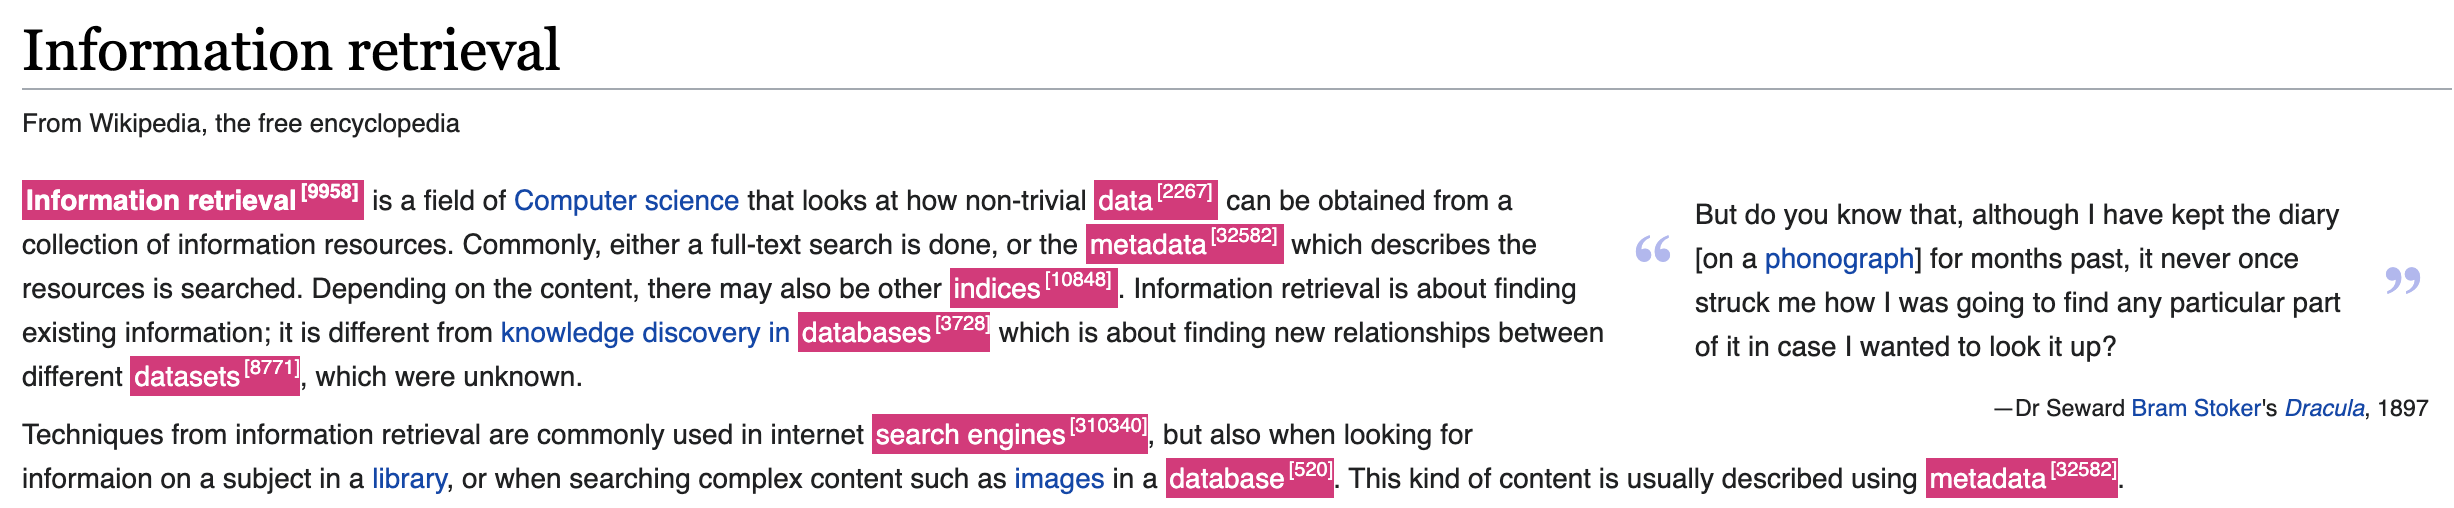
\includegraphics[width=\textwidth]{pictures/concept_annotation_example.png}
     \caption{An example of concept annotations, collected using our annotation tool.}
    \label{fig:concept_annotation_example}
\end{figure}

\section{Simplification as Retrieval Error Analysis Examples} \label{app:retrieval_errors}

In Chapter 6, we show a partial example of aligned Newsela articles that significantly alter content. Here, we show the full text of several such ($D_{i4}$, $D_{i0}$) document pairs, where $D_{i0}$ was ranked outside the top 500 most similar documents. We show two document pairs missed by our BERT-based retrieval method, and one document pair missed by our SBERT-based retrieval method.

\begin{table*}
\begin{center}
\begin{tabular}{|L{14.7cm}|}\hline
\multicolumn{1}{|c|}{\textbf{Source L4 Document}} \\ \hline
\tiny Facebook Chief Executive Mark Zuckerberg announced Tuesday that he plans to eventually donate 99 percent of the Facebook stock owned by him and his wife, Priscilla Chan, shares that are worth about \$45 billion today. That amount would make it one of the largest philanthropic commitments ever.

Zuckerberg said in an open letter that the birth last week of their first child, a daughter named Max, was the motivation to dedicate their considerable wealth to charitable causes now. They wrote that they did not want to wait to ``advance human potential and promote equality for all children."

``I will continue to serve as Facebook's CEO for many, many years to come," Zuckerberg wrote, ``but these issues are too important to wait until you or we are older to begin this work."

The money will be channeled into the Chan Zuckerberg Initiative, a newly formed group that initially will focus on education and health. It was also clear from Zuckerberg's letter that he and his wife had learned lessons from earlier philanthropic attempts and will move in a new direction.

Zuckerberg's announcement stands out because of his relative youth -- he's just 31 -- and the gift's massive size. The donation also comes at a time when the world's wealthiest business leaders seem to be challenging one another to give away their fortunes before they die.

In 2010, Bill Gates and Warren Buffett publicly launched the Giving Pledge to encourage billionaires to donate the bulk of their wealth to charity. Gates, the former Microsoft leader, has already donated \$31.5 billion, mostly to the Bill and Melinda Gates Foundation. Buffett has donated more than \$22 billion of his Berkshire Hathaway stock and plans to give away nearly his entire fortune.

More than 130 billionaires worldwide have joined them, including Judy Faulkner, founder of the electronic health-records company Epic, who reportedly said she plans to give away 99 percent of her money. Also this year, Saudi Arabia's Prince Alwaleed bin Talal, one of the richest men in the world, said the pledge inspired him to eventually give away his entire fortune, more than \$30 billion.

Zuckerberg quietly committed weeks ago to this pledge, too, although his Nov. 9 Giving Pledge letter didn't reveal the scale of his intentions.

A federal filing shows the Facebook co-founder will start by giving away up to \$1 billion a year in Facebook stock for the first three years. Such tax-efficient arrangements are not unusual for gifts to private foundations.

``He clearly wants to be perceived as a leader of his generation in the same way as Buffett and Gates are theirs," said Richard Marker of the New York advisory firm Wise Philanthropy.

The couple revealed their plans in a lengthy ``letter to our daughter" published on Facebook, the social network that Zuckerberg co-founded while a student at Harvard University and that today has 1.5 billion monthly active users worldwide.

Their daughter's full name is Maxima Chan Zuckerberg, and she was born just before Thanksgiving, weighing 7 pounds, 8 ounces, according to a Facebook spokeswoman.

In the open letter, Zuckerberg and Chan talked about the potential that technology offers to re-engineer the way children learn.

``Our generation grew up in classrooms where we all learned the same things at the same pace regardless of our interests or needs," they wrote.

Zuckerberg and Chan have given \$15 million to AltSchool, a for-profit corporation founded by a former Google executive that works to create a network of schools that use technology to personalize instruction. The couple also has given \$120 million to traditional public schools and public charter schools in the San Francisco area.

But Zuckerberg's first foray into education philanthropy was in itself a learning experience. In 2010, he gave \$100 million to remake public schools in Newark, New Jersey, with mixed results.

Critics of that effort said the plan faltered in part because it was a top-down approach that called for wholesale changes in the city's public schools with plans crafted by outsiders, not community members.

In their letter to Max, Zuckerberg and Chan talked about learning from mistakes.

``Your mother and I have both taught students and we've seen what it takes to make this work. It will take working with the strongest leaders in education to help schools around the world adopt personalized learning. It will take engaging with communities, which is why we're starting in our San Francisco Bay Area community."

Zuckerberg and Chan, a pediatrician and onetime teacher, plan to open a private, tuition-free school for low-income children in East Palo Alto, California, that will integrate health care and support for families with classroom learning.

Although the letter to Max was obviously intended for a wide audience, revealing their ambition to fund billions of dollars in new philanthropic works, the couple ended the note in a personal, quiet fashion.

It was signed simply: ``Love, Mom and Dad." \\ \hline \hline
\multicolumn{1}{|c|}{\textbf{Missed Aligned L0 Document}} \\ \hline 
\tiny Mark Zuckerberg runs Facebook. He helped start the company when he was a in college.

Facebook is used by billions of people around the world. It has made Mark a great deal of money. He is very, very rich.

Mark had some big news his week. He said he and his wife will give away much of their money. His wife's name is Priscilla Chan. She is a doctor.

The two promised to give away around \$45 billion. The money will be used to help make schools better.

\#\# News Was Delivered On Facebook

Mark said this on Facebook. It was in a letter to his first child. Her name is Maxima Chan Zuckerberg.

Maxima was born in November. Her mother and father call her Max for short.

Mark said it was time to start giving to others. He and his wife want to help all children be the best they can be.

Mark and Priscilla said computers can make schools better. They can help kids learn. There are many new ideas on how to use computers and other technology.

\#\# Learning That Fits Each Student

The two said they ``grew up in classrooms where we all learned the same things." Some students learned more quickly than others. Students were interested in different things. Everyone learned the same things in the same way.

Teaching that way can be a problem, they said. Some students do not do as well as they can. Others are bored.

\#\# Better Teaching With Technology

Technology can make teaching better, Mark and Priscilla said. It makes teaching different for each student. All kids learn in the way that is best for them.

The money Mark and Priscilla are giving away will help schools use new technology. It will help them to do better in school.

Mark and Priscilla are also opening a free school for poor children. The school will be in California. \\ \hline
\end{tabular}
\end{center}
\caption{\label{table:example1} Example 1 of an aligned document pair missed by our BERT-based model, titled \textit{zuckerberg-donation}.}
\end{table*}

\begin{table*}
\begin{center}
\begin{tabular}{|L{14.7cm}|}\hline
\multicolumn{1}{|c|}{\textbf{Source L4 Document}} \\ \hline
\tiny ANCHORAGE - Anna Oxereok grew up eating walrus in the western Alaska village of Wales. Today it's such a rare treat she can't bring herself to part with the plastic gallon bag of meat in her freezer.

``I have to save it for something special," she says.

Her brother caught two animals this spring and shared the meat and fat, but it didn't go very far in the village of 150. She is thankful for what she got, though. It's become increasingly difficult to land a walrus.

Other remote communities at the edge of the Bering Sea also are seeing a steep decline in walrus harvested the past several years. Walrus, described by some as having a taste between veal and beef, is highly prized by Alaska Natives as a subsistence food to store for winter, with the adult male animals averaging 2,700 pounds. The sale of carved ivory from the tusks, legal only for Alaska Natives, also brings in supplemental income to communities with high unemployment rates.

Hunters and scientists say walrus migration patterns are veering from historical hunting grounds as temperatures rise and the ocean ice used by the animals to dive and rest recedes farther north. Village elders also tell biologists the wind is blowing in new directions. In 2013, a late-season icepack clustered around St. Lawrence Island, blocking hunters from the sea.

``I think one of the biggest issues is that things have gotten so variable. It's hard to really predict what's going to happen," said Jim MacCracken, Alaska walrus program supervisor for the U.S. Fish and Wildlife Service.

Iver Campbell and other Yup'ik Eskimo hunters from two St. Lawrence Island communities harvested more than 1,100 walrus in 2003. But a decade later, hunters managed to take only 555 - a fraction of the ideal of one walrus per resident, per year. Things still are not looking any better for the 1,430 residents of the villages of Gambell and Savoonga. The recent spring take was 233 walrus, according to preliminary Fish and Wildlife figures.

The shore ice once served to block the wind for hunters but that's no longer the case, said Campbell, who has lived all 64 years in Gambell, population 713.

``The ice goes out real fast, melts real fast," he said. ``We don't have anything to counter the wind and the rough water."

Science backs that observation. According to the Office of Naval Research, the past eight years have had the eight lowest amounts of summer sea ice on record.

Far from the state's limited road system, costly store-bought food is not an affordable solution. At village stores, pantry staples quickly add up - nearly \$7 for a dozen eggs, \$15 for a gallon of milk and \$6.25 for a loaf of basic white bread. People rely on the region's resources for up to 80 percent of their diets.

Their hunting practices are closely monitored by federal authorities to ensure the animals that are killed are not going to waste. Generally, such hunts do not cause a public outcry in Alaska.

In these communities, a subsistence lifestyle is a necessity. In fact, the low harvest this year recently prompted a donation of 10,000 pounds of frozen halibut to four affected villages.

``A decline in the subsistence harvest really creates an economic disaster that threatens the health and welfare of the people in the communities," said Vera Metcalf, director of the Eskimo Walrus Commission. ``So we are concerned about the impacts of climate change and the ability for our hunters to harvest marine mammals."

Some Native communities can search for other animals, like domestic reindeer or caribou. But opportunities aren't as bountiful for Diomede on the western coast of Little Diomede Island, only a few miles from Russia. The community of 120 harvested one walrus in 2014, prompting city and Native leaders to seek assistance from the state.

This year, 10 walrus were harvested, according to Diomede hunter Robert Soolook. There's no shortage of walrus, he said, but they are migrating sooner. No one has initiated any long-range planning to address the shift, but Soolook believes hunters eventually will need to change their practices, even going out earlier.

``Now that we've seen this, we have to start adapting," he said.

No federal assistance is available, and state aid is minimal, at best. State Sen. Donny Olson, a Democrat from Golovin, said he might introduce legislation to allow failed subsistence hunts to qualify for state disaster funds.

Moving from her ancestral lands is not an option, according to Oxereok, an Inupiat Eskimo. Relocating would mean displacing everything she knows.

``It's not that simple because your roots are here," she said. \\ \hline \hline
\multicolumn{1}{|c|}{\textbf{Missed Aligned L0 Document}} \\ \hline 
\tiny ANCHORAGE, Alaska - There are people who have been living in Alaska for many, many years. They were living there long before the United States began. They are called Native Alaskans.

Native Alaskans eat walrus. Walrus are large sea animals. Only Native Alaskans are allowed to hunt walrus. Eating walrus is part of their way of life.

These days, walrus are hard to find. There are not as many in Alaska anymore. Global warming has made many walrus swim away. The ice they like is melting. Global warming means that our planet is getting hotter.

\#\# A Special Piece Of Meat

If there are no walrus to eat, Native Alaskans will not have enough food. Some people are going hungry.

Anna Oxereok is a Native Alaskan. She grew up eating walrus in her village. Today, she does not eat much walrus. Anna has one piece of walrus in her freezer. She is waiting to eat it.

``I have to save it for something special," she says.

Her brother caught two walrus this spring. He shared them with their village. Two walrus for 150 people was not very much. Anna was glad she got some.

\#\# Walrus Look For Ice

Walrus are moving around more. Global warming has forced them to. In Alaska, there is ice in the sea. Walrus like to rest on the ice. Now it is getting warmer in Alaska. More ice has turned to water. Some walrus have moved. They went to where there is still ice. Now there are fewer walrus for Native Alaskans to hunt.

Without walrus to eat, there has been less meat. Native Alaskans do not buy much food in stores. They do not have enough money. They must find their own food. Finding enough food has been hard without walrus.

Anna is not thinking about moving. Moving would mean leaving everything she knows. Anna will stay. She hopes that enough walrus stay, too. \\ \hline
\end{tabular}
\end{center}
\caption{\label{table:example2} Example 2 of an aligned document pair missed by our BERT-based model, titled \textit{walrus-alaska}.}
\end{table*}

\begin{table*}
\begin{center}
\begin{tabular}{|L{14.7cm}|}\hline
\multicolumn{1}{|c|}{\textbf{Source L4 Document}} \\ \hline
\tiny WASHINGTON - As proof that he can successfully and humanely deport the estimated 11 million people living in the country illegally, Republican presidential contender Donald Trump often touts the efforts of the Eisenhower administration in the 1950s.

He did so again during the Republican debate on Nov. 10, saying ``you don't get nicer, you don't get friendlier" than President Dwight D. Eisenhower. ``They moved 1.5 million out," the billionaire real estate mogul said. ``We have no choice. We have no choice."

But the program to which Trump refers, known as ``Operation Wetback," was a complicated undertaking largely viewed by historians as a dark moment in America's past. Also lost in Trump's telling is that it coincided with a guest worker program that provided legal status to hundreds of thousands of largely Mexican farm workers.

Trump declined to refer to the program by name on Nov. 11 in an interview on The O'Reilly Factor. ``I don't like the term at all," he said.

But he nonetheless defended what host Bill O'Reilly described as brutal treatment of those who were deported.

``I've heard it both ways. I've heard good reports, I've heard bad reports," Trump said. ``We would do it in a very humane way."

``He's only got part of the story," said Mae Ngai, a professor of history at Columbia University.

The operation was named after a term for Mexicans who crossed the Rio Grande that is now viewed a racial slur. The 1954 initiative was aimed at apprehending and deporting agricultural workers who had crossed the border illegally looking for work.

According to a summary of the project from the Texas State Historical Association, the United States Border Patrol ``aided by municipal, county, state, and federal authorities, as well as the military, began a quasi-military operation of search and seizure of all unauthorized immigrants."

The project, Ngai said, began with 750 immigration officers and border control agents, who used jeeps, trucks, buses and airplanes to apprehend migrants nationwide, including in Los Angeles, San Francisco and Chicago. They apprehended 3,000 people a day and 170,000 during its first three months.

In an interview on Nov. 11 on MSNBC's ``Morning Joe," Trump indicated he would take a similar approach. "You're going to have a deportation force, and you're going to do it humanely," he said.

Critics of the program say the conditions for those the agents apprehended were anything but humane. Many of the apprehended migrants were transported in crowded buses and dumped on the other side of the border in a manner that some at the time equated with the treatment of livestock.

In one incident, Ngai said, 88 apprehended Mexicans died of sunstroke after being subjected to 112-degree heat. The number would have been higher had the Red Cross not intervened.

Some of those apprehended were sent deep into the interior of Mexico to prevent re-entry by train or cargo ship, where conditions drew the attention of federal regulators.

One congressional investigation likened a transport ship that was the site of a riot to an ``18th century slave ship" and a ``penal hell ship."

Trump touted the approach as a virtue of the Eisenhower-era program in the Nov. 10 debate.

``Moved a 1.5 million illegal immigrants out of this country, moved them just beyond the border. They came back. Moved them again beyond the border, they came back. Didn't like it," Trump said. "Moved them way south. They never came back."

Trump also leaves out of his advocacy for the Eisenhower-era approach the fact the program was developed to complement a guest-worker program that began in the 1940s and was aimed at allowing Mexican farmworkers to enter the country and work in the United States legally.

Hundreds of thousands of farm workers did so, and the deportation effort was conceived as a way to pressure employers into using the guest worker program.

``It was like a carrot and a stick," Ngai said.

While Trump has put the number of deportations at 1.5 million, most accounts suggest the numbers are far fewer, because they included those who chose to leave the country voluntarily as well as people who returned after being deported and were deported again.

Trump has yet to lay out precisely how he would track down those living in the country illegally, or how he would determine who are ``the good ones" that he would allow to return. Both John Kasich, Ohio's governor, and Jeb Bush, the former governor of Florida, rejected Trump's plan as unrealistic and cruel in the Republican presidential candidates' debate on Tuesday night, Nov. 10.

``To send them back, 500,000 a month, is just not, not possible," Bush said. ``And it's not embracing American values. And it would tear communities apart. And it would send a signal that we're not the kind of country that I know America is." \\ \hline \hline
\multicolumn{1}{|c|}{\textbf{Missed Aligned L0 Document}} \\ \hline 
\tiny WASHINGTON, D.C. - Donald Trump is running for president.

The race for president is in two parts. The first part is known as the primaries. Republican candidates run against other Republicans in the Republican primary. Democrats run against Democrats in the Democratic primary.

Then, the winner of the Republican primary runs against the winner of the Democratic primary. The second race happens in 2016. It is known as the election. The people picked to run in that race are called the nominees. The winner of the election becomes president.

On Nov. 10, Republican candidates got together for a debate. They all said what they would do if elected president. They gave speeches on TV. Trump is a Republican. He said that millions of people are living in the country against the law. He would make them all leave.

\#\# Trump Likes One-Way Trips

Trump praised a program from the 1950s. It forced farmworkers to leave the United States. Most of them were from Mexico. They crossed the border without permission. They were looking for work.

Trump likes the program. He said it was nice and friendly. He called it proof that he could send farmworkers back to their own countries in a kind way.

\#\# Historians Oppose Trump's View

Historians do not agree with Trump. Most of them call the 1950s program an ugly moment in America's past.

The program began with 750 government officers. They used jeeps, trucks, buses and airplanes to find the farm workers. The officers caught 3,000 people a day. They caught about 170,000 during the program's first three months.

Many people say the government treated the farmworkers badly. The government put them on crowded buses. Then they were dumped on the Mexican side of the border.

At one point, 88 Mexicans died, said Mae Ngai, a history professor. The Mexican workers were left outside in very hot weather.

\#\# GOP Rivals Criticize Trump's Plan

Two Republican candidates spoke out against Trump's plan. One of the candidates was Ohio Governor John Kasich. The other one was Jeb Bush. He used to be the governor of Florida. Both of them said Trump's plan was cruel. They also said it would be hard to carry out.

Bush said Trump's plan is against American values. He said that America is a better country than that. \\ \hline
\end{tabular}
\end{center}
\caption{\label{table:example3} Example of an aligned document pair missed by our SBERT-based model, titled \textit{trump-immigration}.}
\end{table*}
